\section{Protecting Against Adversarial Attacks}

    \subsection{Binary Thresholding}

        We’ve just created images that trick neural networks. The next question we could ask is whether or not we could protect against these kinds of attacks. If you look closely at the original images and the adversarial examples you’ll see that the adversarial examples have some sort of grey tinged background.

        \begin{figure}[htbp]
            \centering
            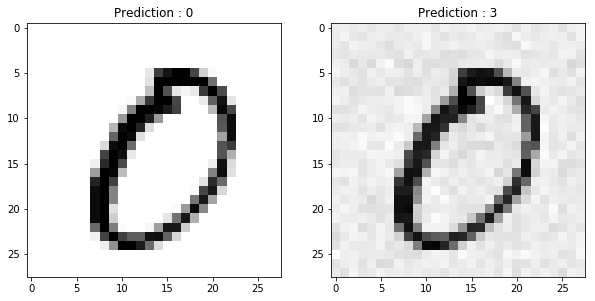
\includegraphics[width=0.7\linewidth]{images/adversarial1.png}
            \caption{Generated Adversarial Image}
        \end{figure}

        \begin{figure}[htbp]
            \centering
            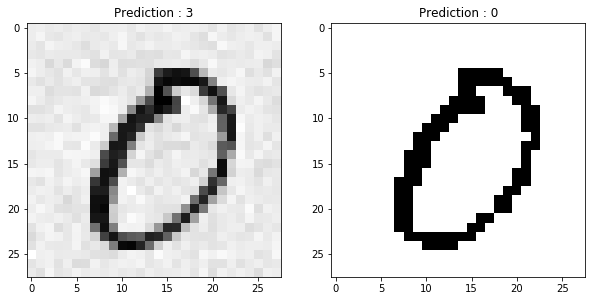
\includegraphics[width=0.7\linewidth]{images/thresholding.png}
            \caption{The effect of binary thresholding on an MNIST adversarial image. The left image is the adversarial image, the right side is the binarized image}
        \end{figure}

        One naive thing we could try is to use binary thresholding to completely white out the background. Turns out binary thresholding works! But this way of protecting against adversarial attacks is not very good. Not all images will always have an all white background. For example in \cref{fig:panda_thresholding},	 panda at the very beginning of this post. Doing binary thresholding on that image might remove the noise, but not without disturbing the image of the panda a ton. Probably to the point where the network (and humans) can’t even tell it’s a panda.
                
        \begin{figure}[htbp]
            \centering
            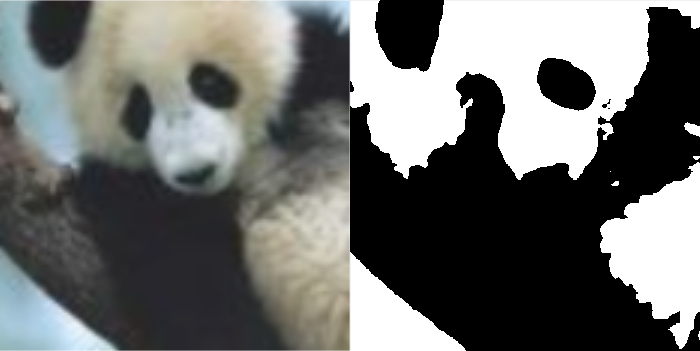
\includegraphics[width=0.7\linewidth]{images/panda_thresholding.png}
            \caption{Doing binary thresholding on the panda results in a blobby image}
            \label{fig:panda_thresholding}
        \end{figure}

    \subsection{Adversarial training}
        One of the easiest and most brute-force way to defend against these attacks is to pretend to be the attacker, generate a number of adversarial examples against your own network, and then explicitly train the model to not be fooled by them. This improves the generalization of the model but hasn’t been able to provide a meaningful level of robustness — in fact, it just ends up being a game of whack-a-mole where attackers and defenders are just trying to one-up each other.

    \subsection{Defensive distillation}
        In defensive distillation, we train a secondary model whose surface is smoothed in the directions an attacker will typically try to exploit, making it difficult for them to discover adversarial input tweaks that lead to incorrect categorization. The reason it works is that unlike the first model, the second model is trained on the primary model’s “soft” probability outputs, rather than the “hard” (0/1) true labels from the real training data. This technique was shown to have some success defending initial variants of adversarial attacks but has been beaten by more recent ones, like the Carlini-Wagner attack, which is the current benchmark for evaluating the robustness of a neural network against adversarial attacks.

    \subsection{Why is defending neural networks so hard?}
        Let’s try to develop an intuition behind what’s going on here. Most of the time, machine learning models work very well but only work on a very small amount of all the many possible inputs they might encounter. In a high-dimensional space, a very small perturbation in each individual input pixel can be enough to cause a dramatic change in the dot products down the neural network. So, it’s very easy to nudge the input image to a point in high-dimensional space that our networks have never seen before. This is a key point to keep in mind: the high dimensional spaces are so sparse that most of our training data is concentrated in a very small region known as the manifold. Although our neural networks are nonlinear by definition, the most common activation function we use to train them, the Rectifier Linear Unit, or ReLu, is linear for inputs greater than $0$.

        \begin{figure}[htbp]
            \centering
            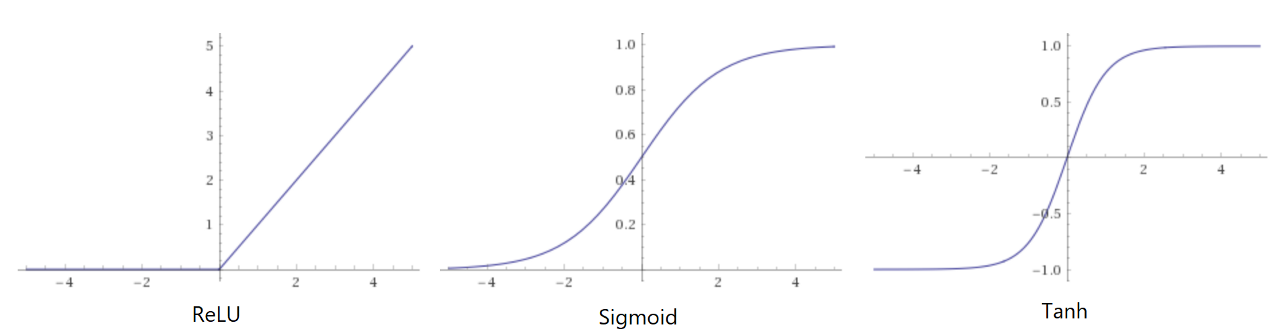
\includegraphics[width=\linewidth]{images/functions.png}
            \caption{The Rectifier Linear Unit, or the ReLu compared to the Sigmoid and the Tanh activation functions.}
        \end{figure}

        ReLu became the preferred activations function due to its ease of trainability. Compared to sigmoid or tanh activation functions that simply saturate to a capped value at high activations and thus have gradients getting “stuck” very close to $0$, the ReLu has a non-zero gradient everywhere to the right of $0$, making it much more stable and faster to train. But, that also makes it possible to push the ReLu activation function to arbitrarily high values.

        Looking at this trade-off between trainability and robustness to adversarial attacks, we can conclude that the neural network models we have been using are intrinsically flawed. Ease of optimization has come at the cost of models that are easily misled.		
